\documentclass{proc}

\usepackage[margin=2cm]{geometry}
\usepackage{graphicx}

\title{Including graphics}
\author{Author}
\date{}

\begin{document}
    \maketitle

    \section{Introduction}

        Picture books are just \emph{better}.

        \subsection{Include graphics}

        This is a banana in a JPG.

        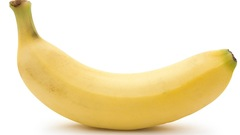
\includegraphics[width=2in]{src/examples/assets/img/Banana.jpg} % Use relative paths to working directory or to inputs specified with --input (desciption in /README.md#command-line-options)

        This is a fish, in chart, in a PNG.

        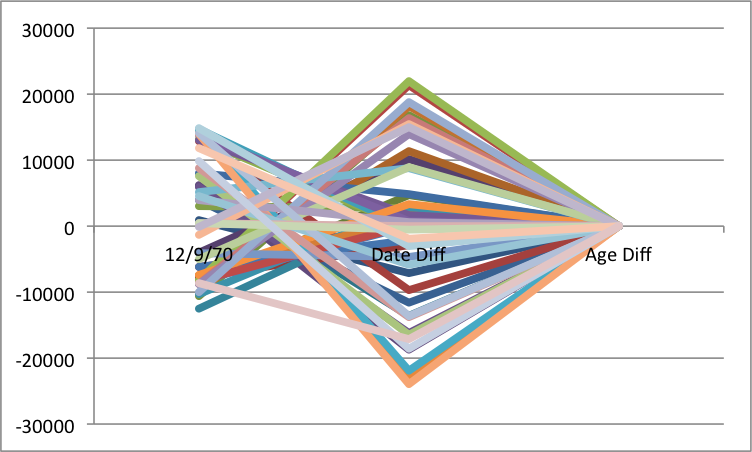
\includegraphics[width=2in]{src/examples/assets/img/Fish.png}

        \subsection{Float: Figure environment}

        In my article, I want to include a JPG image of a banana. You can see this image in Figure~\ref{fig:banana}.

        \begin{figure}[htbp]
            \begin{center}
                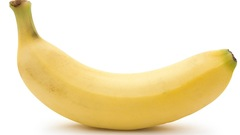
\includegraphics[width=2in]{src/examples/assets/img/Banana.jpg}
                \caption{This is a banana.}
            \end{center}
            \label{fig:banana}
        \end{figure}

        In my article, I want to include a PNG image of a chart that looks like a fish. You can see this image in Figure~\ref{fig:fish}

        \begin{figure}[htbp]
            \begin{center}
                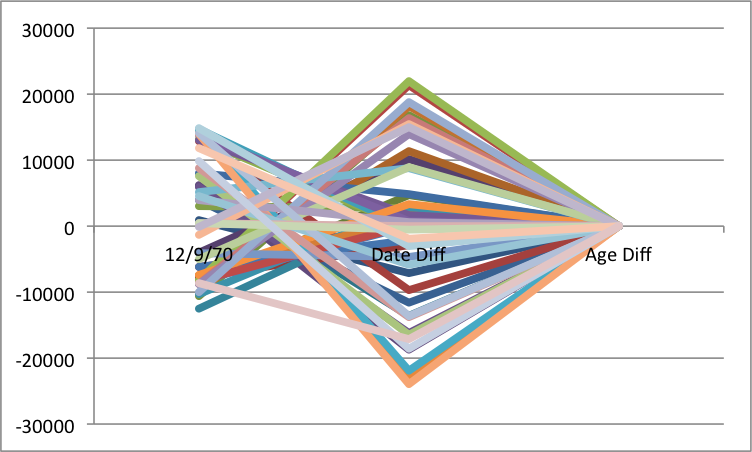
\includegraphics[width=2in]{src/examples/assets/img/Fish.png}
                \caption{This is chart that looks like a fish.}
            \end{center}
            \label{fig:fish}
        \end{figure}


    \section{Conclusion}

    Adding images to an article.

\end{document}
